\documentclass[12pt, french]{article}

\usepackage{fancyhdr, fancybox, lastpage,mhchem}
\usepackage[most]{tcolorbox}
\usepackage[a4paper, margin={0.3in, .75in}]{geometry}
\usepackage{wrapfig}
\pagestyle{fancy}
\renewcommand\headrulewidth{1pt}
\renewcommand\footrulewidth{1pt}
\fancyhf{}
\rhead{ \em{Zakaria Haouzan}}
\lhead[C]{\em{2ème année baccalauréat Sciences Mathématiques}}
\chead[C]{}
\rfoot[C]{}
\lfoot[R]{}
\cfoot[]{\em{Page \thepage / \pageref{LastPage}}}


\newtcolorbox{Box2}[2][
enhanced,
breakable,
]{
                lower separated=false,
                colback=white,
colframe=white!20!black,fonttitle=\bfseries,
colbacktitle=white!30!gray,
coltitle=black,
enhanced,
attach boxed title to top left={yshift=-0.1in,xshift=0.15in},
title=#2,#1}


\begin{document}
\begin{center}
   \shadowbox {\bf{Transformations chimique qui s’effectuent en deux sens
}
 }

\end{center}

\vspace{-0.2cm}
%%_________________________Exercice ! :"_________________________Exercice
   \begin{Box2}{Exercice 1 :  Acide chlorhydrique}
	On considère un mélange de :

	-Une solution $S_1$ d’acide chlorhydrique de volume $V_1 =5mL$ et de concentration molaire $C_1=0.5mol/L$

	-Une solution $S_2$ d’acide chlorhydrique de volume $V_1 =20mL$ et $pH=1.3$

1. Ecrire l'équation de la réaction chimique d’acide chlorhydrique et l’eau

2. Calculer la quantité de la matière de H3O+ pour chaque solution ? déduire la concentration molaire du
mélange ?

3. Calculer le pH du mélange ?

   \end{Box2}


%%_________________________Exercice !2 :"_________________________Exercice
\begin{Box2}{Exercice 2 :}
%\begin{wrapfigure}{r}{0.22\textwidth}
  %\begin{center}
	  %\vspace{-0.6cm}
	%\includegraphics[width=0.22\textwidth]{./img/Ex2.png}
  %\end{center}
%\end{wrapfigure}

	Le pH de la solution d’acide méthanoïque $HCOOH$ de concentration $C=1,0.10^{-1}moL/L$ est $pH=2.4$

1. Ecrire l'équation de la réaction chimique d’acide méthanoïque avec l’eau ?

2. Dresser le tableau d'avancement de la réaction chimique ?

3. Montrer que la réaction chimique n’est pas totale ?

4. Calculer les concentrations molaires finales des ions de la solution à l’état final de la réaction chimique? (on
néglige les ions $HO^-$)


\end{Box2}

%%_________________________Exercice ! 3:"_________________________Exercice
\begin{Box2}{Exercice 3 : }
%\begin{wrapfigure}{r}{0.5\textwidth}
  %\begin{center}
	%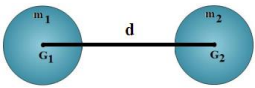
\includegraphics[width=0.5\textwidth]{./img/ex3.png}
  %\end{center}
%\end{wrapfigure}
	Le pH d’une solution aqueuse d’ibuprofène $C_{13}H_{18}O_2$ de concentration molaire $C = 5,0.10^{-2} mol.L^{-1}$ vaut $pH = 2,7$
	à $25^{\circ}C$.

1. Ecrire l'équation de la réaction modélisant la transformation entre l’ibuprofène et l'eau

2. Déterminer l’avancement final $x_f$ en fonction de pH et V

3. Déterminer xm en fonction C et V

4. Montrer que cette transformation est limitée.


\end{Box2}

%%_________________________Exercice 4 : _________________________Exercice
\begin{Box2}{Exercice 4 : }
   % \begin{wrapfigure}[12]{r}{0.5\textwidth}
  %\begin{center}
	  %\vspace{-0.6cm}
	%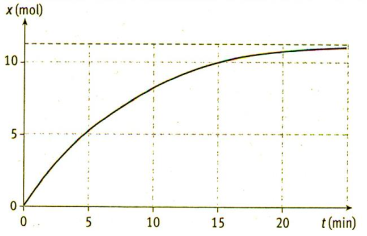
\includegraphics[width=0.5\textwidth]{./img/ex4.png}
  %\end{center}
%\end{wrapfigure}
L'acide propanoïque $C_2H_5COOH$ est un acide gras, utilisé dans la synthèse de certains produits organiques et
pharmaceutiques, de parfums et dans la médecine vétérinaire.

1. On considère, à 25°C, une solution aqueuse (S) d’acide propanoïque de concentration molaire $C =2,0.10^{-3}mol.L^{-1}$ et de volume $V =1,0 L$. La mesure de la conductivité $\sigma$ de la solution (S) a donné la valeur $\sigma = 6,2.10^{-3} S.m^{-1}$.
$$\lambda_{H_3O^+} = 35.10^{-3}S.m^2/mol \hspace{1cm} \lambda_{C_2H_5COO^-}=3,58.10^{-3}S.m^2/mol$$

1.1. Écrire l’équation chimique modélisant la réaction de l’acide propanoïque avec l’eau.

1.2. Dresser le tableau d’avancement de la réaction en utilisant les grandeurs $C_A$, $V_A$, l'avancement $x$ et l'avancement $x_{eq}$ à l'état d’équilibre du système chimique. Déterminer la valeur de l'avancement maximal.

1.3. Vérifier que la valeur de l'avancement à l'état d’équilibre est $1, 6.10^{-4} mol$ .

1.4. Calculer la valeur du taux d'avancement final.

2- On considère une solution aqueuse (S') d'acide propanoïque de concentration molaire $C_A$=$2.10^{-4} mol.L^{-1}$ et de
$pH = 4, 3$ . On note $\tau'$ le taux d'avancement final de la réaction de l'acide propanoïque avec l'eau dans ce cas.

2.1. Déterminer la valeur de $\tau'$ .

2.2. Comparer les valeurs de $\tau$ et $\tau'$ . Déduire.


\end{Box2}


\begin{center}

\shadowbox{ 	   \bf{Etat d'équilibre d'un système chimique}}
\end{center}


\vspace{-0.6cm}
%%_________________________Exercice 5 : _________________________Exercice
\begin{Box2}{Exercice 4 : }
   % \begin{wrapfigure}[14]{r}{0.5\textwidth}
  %\begin{center}
	  %\vspace{-0.6cm}
	%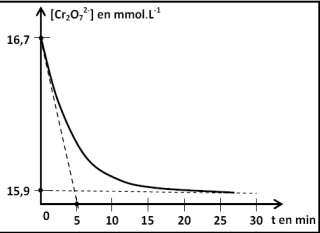
\includegraphics[width=0.5\textwidth]{./img/ex5.png}
  %\end{center}
%\end{wrapfigure}
	On considère une solution $(S_a)$ d’acide méthanoïque de volume V et de concentration molaire $C_a$=$ 10^{-2} mol/L$.
La mesure du pH de cette solution donne : $pH = 2,9$.
On modélise la réaction entre l’acide méthanoïque et l’eau par l’équation suivante :
\vspace{-0.4cm}
$$\ce{HCOOH_{(aq)} + H_2O_{(aq)} <=> HCOO^-_{(aq)} + H_3O^+_{(aq)} }$$

1. Construire le tableau d’avancement de l’évolution du système.

2. Montrer que le taux d’avancement final de cette transformation s’écrit sous la forme $\tau $=$ \frac{10^{-pH}}{C_a}$.Calculer la valeur de $\tau$, et conclure.

\end{Box2}

\begin{Box2}{Exercice 5 : }
On note l’acide Ibuprofène par RCOOH et sa base conjuguée par $RCOO^-$. $M(RCOO^-) = 206g/mol$.

On dissout, dans l'eau pure, un échantillon de masse $m = 200 mg$ d'acide $RCOOH$, contenu dans un sachet
d'Ibuprofène, pour obtenir une solution aqueuse $(S_0)$ de concentration $C_0$ et de volume $V0 $=$ 100 mL$.

1.1. Calculer $C_0$.

1.2. La mesure du pH de la solution $S_0$ a donné la valeur : $pH = 3,17$.

1.2.1 Vérifier, à l'aide du tableau d'avancement, que la réaction de l’Ibuprofène avec l'eau est limitée.

\end{Box2}


\begin{Box2}{Exercice 6 : }

On désignera l’acide étudié par AH et sa base conjuguée par $A^-$ 

On prépare une solution (SA) d’acide butanoïque de concentration molaire $C_A$=$ 10^{-2} mol/L$ et de volume $V_A$.
La mesure du pH de la solution $(S_A)$ donne $pH = 3,41$.

1. Construire le tableau d’avancement.

2. Donner l’expression de l’avancement $x_{eq}$ à l’équilibre en fonction de $V_A$ et $[H_3O^+]_{eq}$ (Concentration molaire
des ions hydroniums à l’équilibre)

3. Trouver l’expression du taux d’avancement final $\tau$ à l’équilibre en fonction de $pH$ et $C_A$, puis calculer sa
valeur. Que conclure ?


\end{Box2}


\begin{Box2}{Exercice 7 : }
	Les conductivités molaires ioniques : $\lambda_{H_3O^+}$=$3,49.10^{-2}S.m^2/mol$ ; $\lambda_{CH_3COO^-}$=$4,09.10^{-3}S.m^2/mol$

	On dispose de deux solutions (S1) et (S2) d’acide éthanoïque.

	La conductivité de la solution (S1) de concentration molaire $C_1=5.10^{-2}mol/L$ ; $\sigma_1= 3,5.10^{-2}S/m$.

	La conductivité de la solution (S2) de concentration molaire $C_2=5.10^{-3}mol/L$ ; $\sigma_2=1,1.10^{-2}S/m$.

	On considère que la dissolution de l’acide éthanoïque dans l’eau est limitée.

1. Ecrire l’équation modélisant la dissolution de l’acide éthanoïque dans l’eau.

2. Trouver l’expression de la concentration molaire effective $[H_3O^+]_{(eq)}$ des ions oxoniums à l’équilibre en
fonction de $\sigma$ et $\lambda_{CH_3COO^-}$ et $\lambda_{H_3O^+}$.

3. Calculer $[H_3O^+]_{(eq)}$ dans chacune des solutions (S1) et (S2).

4. Déterminer les taux d’avancement final $\tau_1$ et $\tau_2$ de la réaction de l’acide éthanoïque avec l’eau dans chacune
des solutions (S1) et (S2). Déduire l’influence de la concentration initiale de la solution sur le taux
d’avancement final.

\end{Box2}
\begin{center}
   \Large{ \em{Exercices Supplémentaires}}

\end{center}

\begin{Box2}{Exercice 1 : Équilibre chimique dans une solution aqueuse}
  Soit une solution aqueuse contenant du sulfure d’hydrogène $H_2S$, des ions hydrogénosulfure $HS^-$, des ions phénolate $C_6 H_5O^-$, du phénol $C_6H_5OH$, et des ions sodium $Na^+$. Ce système peut être le siège de la réaction chimique d’équation :

  $\ce{H_2 S(aq) + C_6 H_5 O^- (aq) <=> HS^- (aq) + C_6 H_5 OH (aq)}$

Sa composition initiale est donnée ci-dessous :

\[
[H_2 S]_0 = 0, 0100 \, 
  \text{mol} \cdot \text{L}^{-1}; \quad [HS^-]_0 = 0,0200 \, \text{mol} \cdot \text{L}^{-1}; \quad [C_6 H_5 O^-]_0 = 0,0050 \, \text{mol} \cdot \text{L}^{-1};
  \]

  \[
  \quad [C_6 H_5 OH]_0 = 0,0050 \, \text{mol} \cdot \text{L}^{-1}
\]
1. Donner l’expression littérale du quotient de réaction correspondant.\\
2. Calculer sa valeur :
   \begin{itemize}
       \item[(a)] Dans l’état initial du système ;
       \item[(b)] Dans l’état du système tel que $[HS^-] = 0,0230$ mol.L$^{-1}$.
   \end{itemize}
\end{Box2}



\begin{Box2}{Exercice 2 : Dissolution de l’iodure de plomb}
On introduit $4,61$ g d’iodure de plomb solide $PbI_2$ dans $1,00$ L d’une solution d’iodure de potassium, $K^+ + I^-$, de concentration $1,0 \times 10^{-4}$ mol.L$^{-1}$. On suppose que l’introduction du solide ne modifie pas le volume de la solution.

1. L’iodure de plomb peut se dissoudre dans l’eau pour donner des ions iodure $I^-$ et plomb (II) $Pb^{2+}$. Écrire l’équation de cette dissolution avec un nombre stœchiométrique égal à 1 pour l’iodure de plomb.\\

2. Donner l’expression du quotient de réaction correspondant.\\

3. Déterminer sa valeur :
   \begin{itemize}
       \item[(a)] dans l’état initial du système considéré ;
       \item[(b)] dans l’état du système tel que $[I^-] = 1,0 \times 10^{-3}$ mol.L$^{-1}$.
   \end{itemize}
\end{Box2}


\begin{Box2}{Exercice 3 : Solution aqueuse d’acide hypochloreux}
Une solution aqueuse, de volume $V = 250$ mL, a été préparée en dissolvant une quantité $n_0 = 1,5$ mmol d’acide hypochloreux $HClO$ dans le volume d’eau distillée nécessaire. L’acide hypochloreux réagit avec l’eau selon la réaction d’équation :
\[
  \ce{{HClO}_{(aq)} + {H_2O}_{(l)} <=> {ClO^-}_{(aq)} + {H_3O^+}_{(aq)}}
\]

1. Donner l’expression du quotient de réaction correspondant.\\

2. Quelle est la valeur du quotient de réaction dans l’état initial du système ?\\

3. Lorsque le système n’évolue plus, la concentration en ion hypochlorite $ClO^-$ vaut $1,4 \times 10^{-5}$ mol.L$^{-1}$. Déterminer la valeur correspondante du quotient de réaction.\\

4. Quelle est la valeur de la constante d’équilibre associée à cette équation ?
\end{Box2}

\begin{Box2}{Exercice 4 : Taux d’avancement final}
L’acide chloroacétique peut réagir avec l’eau selon la réaction d’équation :
\[
  \ce{
\text{ClCH}_2\text{CO}_2\text{H (aq)} + \text{H}_2\text{O (l)} <=>\text{ClCH}_2\text{CO}_2^- \text{ (aq)} + \text{H}_3\text{O}^+ \text{ (aq)}
  }
\]

1. Donner l’expression de la constante d’équilibre associée à cette équation.\\

2. Lorsqu’on introduit $n_0 = 0,0100$ mol d’acide chloroacétique dans de l’eau distillée de façon à obtenir $V_0 = 100$ mL de solution, l’avancement de la réaction vaut $x_{1f} = 1,06$ mmol lorsque le système n’évolue plus.
   \begin{itemize}
       \item[(a)] Donner la composition finale du système.
       \item[(b)] En déduire la valeur de la constante d’équilibre associée à l’équation de la réaction.
       \item[(c)] Déterminer le taux d’avancement final $\tau$ de la réaction.
   \end{itemize}

3. On dilue dix fois, avec de l’eau distillée, la solution précédemment obtenue. La concentration en ion chloroacétate $\text{ClCH}_2 \text{CO}_2^-$ vaut alors $\left[\text{ClCH}_2\text{CO}_2^-\right] = 2,97 \times 10^{-3}$ mol.L$^{-1}$ lorsque ce nouveau système n’évolue plus.
   \begin{itemize}
       \item[(a)] Quel est le volume $V$ de la solution ainsi préparée ?
       \item[(b)] En déduire, pour ce système, l’avancement final de la réaction de l’acide chloroacétique avec l’eau.
       \item[(c)] Quel est le taux d’avancement final correspondant ?
       \item[(d)] Que peut-on en conclure ?
   \end{itemize}

\end{Box2}

\begin{Box2}{Exercice 5 : Acide nitreux}
On considère trois solutions aqueuses $S_1$, $S_2$ et $S_3$ d’acide nitreux $HNO_2$ de concentrations molaires apportées respectives :
\[
C_1 = 1,0 \times 10^{-1} \, \text{mol} \cdot \text{L}^{-1}, \quad C_2 = 1,0 \times 10^{-2} \, \text{mol} \cdot \text{L}^{-1} \quad \text{et} \quad C_3 = 1,0 \times 10^{-5} \, \text{mol} \cdot \text{L}^{-1}
\]

1. Écrire l’équation de la réaction entre l’acide nitreux et l’eau.\\

2. La mesure du pH de ces trois solutions conduit aux valeurs suivantes : $pH_1 = 2,1$, $pH_2 = 3,4$ et $pH_3 = 5,0$.
   \begin{itemize}
       \item[(a)] Calculer, dans les trois cas, le taux d’avancement final de la transformation.
       \item[(b)] Le taux d’avancement final dépend-il des conditions initiales ? Dans quel cas, cette transformation peut-elle être considérée comme totale ?
   \end{itemize}

\end{Box2}

\begin{Box2}{Exercice 6 : Diméthylamine}  
1. À 25°C, le pH d’une solution $S_1$ de diméthylamine $(\text{CH}_3)_2 \text{NH}$ de concentration $C_1 = 1,0 \times 10^{-2} \, \text{mol} \cdot \text{L}^{-1}$ vaut $pH_1 = 11,4$.\\  
  \begin{itemize}  
    \item[(a)] Quel est l’acide conjugué de la diméthylamine ?  
    \item[(b)] Écrire l’équation de la réaction acido-basique entre la diméthylamine et l’eau.  
    \item[(c)] Calculer le taux d’avancement final $\tau_1$ de cette réaction. La transformation est-elle totale ?  
  \end{itemize}  

2. À la même température, le pH d’une solution $S_2$ de diméthylamine de concentration $C_2 = 1,0 \times 10^{-5} \, \text{mol} \cdot \text{L}^{-1}$ vaut $pH_2 = 9,0$. Calculer le taux d’avancement final $\tau_2$ de la réaction entre la diméthylamine et l’eau. La transformation est-elle totale ?  

3. À l’aide des résultats des questions 1. et 2., préciser le sens dans lequel évolue le taux d’avancement final lorsque la concentration de la solution diminue.  
\end{Box2}


\begin{Box2}{Exercice 7 : Utilisation de mesures conductimétriques}
La conductivité $\sigma_0$ d’une solution $S_0$ d’acide éthanoïque de concentration molaire $C_0 = 1,00 \, \text{mmol} \cdot \text{L}^{-1}$ vaut $46 \, \mu\text{S} \cdot \text{cm}^{-1}$.

1. Écrire l’équation de la réaction entre l’acide éthanoïque et l’eau.

2. Calculer les concentrations molaires effectives des ions éthanoate et oxonium.

3. Calculer le taux d’avancement final.

4. Déterminer les valeurs de la constante d’acidité et du $pK_A$ du couple $\text{CH}_3 \text{CO}_2 \text{H} - \text{CH}_3 \text{CO}_2^{-}$.

5. On dilue la solution 10 fois pour obtenir un volume $V_1 = 100,0 \, \text{mL}$ de solution $S_1$ de concentration $C_1$.
  \begin{itemize}
    \item[(a)] Déterminer la nouvelle valeur du taux d’avancement final de la réaction.
    \item[(b)] Quelle est la valeur de la conductivité $\sigma_1$ de cette solution ?
  \end{itemize}

Données : conductivités molaires ioniques $\lambda (\text{H}_3 \text{O}^+ ) = 35,0 \, \text{mS} \cdot \text{m}^2 \cdot \text{mol}^{-1}$ ; $\lambda (\text{CH}_3 \text{CO}_2^-) = 4,1 \, \text{mS} \cdot \text{m}^2 \cdot \text{mol}^{-1}$.
\end{Box2}

\begin{Box2}{Exercice 8 : Étude d’une solution d’acide benzoïque. (SM 2008 N)}

L’acide benzoïque $\text{C}_6 \text{H}_5 \text{COOH}$, est utilisé comme produit de conserve dans l’industrie alimentaire. C’est un solide de couleur blanche.

Le but de cette partie est d’étudier la réaction de l’acide benzoïque avec l’eau, et avec une solution d’hydroxyde de sodium. On prépare une solution aqueuse d’acide benzoïque, par dissolution d’un échantillon de masse $m$ de cet acide dans l’eau distillée, pour obtenir un volume $V = 100 \, \text{mL}$ de solution de concentration molaire $c_a = 0,1 \, \text{mol} \cdot \text{L}^{-1}$.

On donne :
\begin{itemize}
    \item Masse molaire d’acide benzoïque : $M = 122 \, \text{g} \cdot \text{mol}^{-1}$.
    \item Produit ionique de l’eau : $K_e = 10^{-14}$.
\end{itemize}

Réaction de l’acide benzoïque avec l’eau :  
On mesure le pH d’une solution d’acide benzoïque à 25°C, on trouve $pH_1 = 2,6$.

1. Calculer la valeur de la masse $m$.
  
2. Écrire l’équation modélisant la réaction de l’acide benzoïque avec l’eau.

3. Construire le tableau descriptif de l’évolution du système, et calculer la valeur du taux d’avancement final $\tau$ de la réaction. Conclure.

4. Donner l’expression du quotient de réaction $Q_{req}$ à l’équilibre en fonction de $pH_1$ et $c_a$. En déduire la valeur de la constante d’acidité $K_A$ du couple $\left( \text{C}_6 \text{H}_5 \text{COOH(aq)} / \text{C}_6 \text{H}_5 \text{COO}^- (\text{aq}) \right)$.
\end{Box2}

\begin{Box2}{Exercice 9 : Étude d’une solution aqueuse d’acide éthanoïque (SM 2015 R)}

On dispose d’une solution aqueuse (SA) d’acide éthanoïque de concentration molaire $C_A$=$ 10^{-2}mol.L^{-1}$.

La mesure de la conductivité de la solution (SA) donne la valeur $\sigma = 1,6 \times 10^{-2} \, \text{S} \cdot \text{m}^{-1}$.

Données :
\begin{itemize}
    \item Toutes les mesures sont effectuées à 25°C.
    \item Conductivité ionique molaire $\lambda_{\text{H}_3\text{O}^+} = 34,9 \, \text{mS} \cdot \text{m}^2 \cdot \text{mol}^{-1}$ et $\lambda_{\text{CH}_3 \text{COO}^-} = 4,09 \, \text{mS} \cdot \text{m}^2 \cdot \text{mol}^{-1}$,
    \item On néglige l’influence des ions $\text{HO}^-$ sur la conductivité de la solution.
\end{itemize}

1. Écrire l’équation modélisant la réaction de l’acide éthanoïque avec l’eau.

2. Montrer que la valeur du pH de la solution (SA) est $pH = 3,4$.

3. Calculer le taux d’avancement final de la réaction.

4. Trouver l’expression de $pK_A$ du couple $\text{CH}_3 \text{COOH(aq)} / \text{CH}_3 \text{COO}^-(\text{aq})$ en fonction du $pH$ de la solution (SA) et de $C_A$. Calculer sa valeur.
\end{Box2}


\begin{Box2}{Exercice : Étude de la conductivité d'une solution d'acide carboxylique}

Les conductivités molaires ioniques en $\text{S} \cdot \text{m}^2 \cdot \text{mol}^{-1}$ à $\Theta = 25^\circ \text{C}$ :
\begin{itemize}
    \item $\lambda_{\text{H}_3\text{O}^+} = 3,5 \times 10^{-2}$,
    \item $\lambda_{\text{A}^-} = 3,23 \times 10^{-3}$.
\end{itemize}

Une bouteille au laboratoire contient une solution aqueuse (S) d’un acide carboxylique AH de concentration molaire $C = 5 \times 10^{-3} \, \text{mol} \cdot \text{L}^{-1}$ et de volume $V = 1 \, \text{L}$.  
Pour reconnaître cet acide, un technicien de laboratoire mesure la conductivité de la solution (S) et trouve la valeur : $\sigma = 2,03 \times 10^{-2} \, \text{S} \cdot \text{m}^{-1}$.

On modélise la transformation ayant lieu entre l’acide AH et l’eau par l’équation chimique suivante :
\[
\text{AH(aq)} + \text{H}_2\text{O(l)} \longrightarrow \text{A}^- (\text{aq}) + \text{H}_3\text{O}^+ (\text{aq})
\]

Recopier sur votre copie le tableau descriptif suivant et le compléter.

\[
\begin{array}{|c|c|c|c|}
\hline
\text{État} & \text{Avancement} & \text{Quantité de matière en mol} \\
\hline
\text{Initial} & x = 0 & \text{AH} = C, \text{A}^- = 0, \text{H}_3\text{O}^+ = 0 \\
\hline
\text{Intermédiaire} & x & \text{AH} = C - x, \text{A}^- = x, \text{H}_3\text{O}^+ = x \\
\hline
\text{Équilibre} & x_{eq} & \text{AH} = C - x_{eq}, \text{A}^- = x_{eq}, \text{H}_3\text{O}^+ = x_{eq} \\
\hline
\end{array}
\]

1. Trouver la valeur de l’avancement $x_{eq}$ à l’équilibre.

2. Calculer la valeur du taux d’avancement final de la réaction étudiée. Conclure.

3. S’assurer que la valeur du pH de la solution (S) est : $pH = 3,27$.

4. Exprimer le quotient de réaction $Q_{r,eq}$ à l’équilibre en fonction de $pH$ et $C$.

5. En déduire la valeur de $pK_A$ du couple (AH/A$^-$) et identifier l’acide étudié.  
Valeur de $pK_A$ de quelques couples (AH/A$^-$) :
\begin{itemize}
    \item AH/A$^-$ : NH$_4^+$/NH$_3$ : 9,2
    \item HF/F$^-$ : 3,2
    \item HClO/HClO$^-$ : 7,3
    \item C$_6$H$_5$COOH/C$_6$H$_5$COO$^-$ : 4,2
\end{itemize}

Laquelle des deux espèces AH et A$^-$ domine dans la solution (S) ? Justifier.

\end{Box2}


\end{document}
